\documentclass[journal]{IEEEtran}
\usepackage{cite}
\usepackage{amsmath}
\usepackage{booktabs}
\usepackage{graphicx}
\usepackage{tikz}
\usetikzlibrary{arrows.meta,positioning,fit,backgrounds}
\usepackage{algorithm}
\usepackage{algpseudocode}
\usepackage[hidelinks]{hyperref}

\begin{document}

\title{Smart Road Guardian AI X: VRU-First, Observability-Aware Risk Fusion for Indian Roads}

\author{
\begin{tabular}[t]{@{}c@{\hspace{1.2cm}}c@{}}
\begin{tabular}[t]{@{}c@{}}
Aditya Ayushman Sahoo\\
Department of Computational Intelligence,\\
School of Computing,\\
~\\
SRM Institute of Science and Technology,\\
Kattankulathur -- 603203\\
adityaasahoo@gmail.com
\end{tabular}
&
\begin{tabular}[t]{@{}c@{}}
Sageengrana S\\
Department of Computational Intelligence,\\
School of Computing,\\
Faculty of Engineering and Technology,\\
SRM Institute of Science and Technology,\\
Kattankulathur -- 603203\\
sageengranadhas@gmail.com
\end{tabular}
\end{tabular}
\thanks{Code, a live demonstration system, and every result in this paper are open at \url{https://github.com/adityaayushman/TRIE} and \url{https://trie-dashboard.vercel.app}.}}

\markboth{Smart Road Guardian AI X}{Sahoo \MakeLowercase{\textit{et al.}}: VRU-First, Observability-Aware Risk Fusion for Indian Roads}

\maketitle

\begin{abstract}
Most road-safety technology assumes crashes must accumulate before a location is flagged, risk belongs to the occupant, and a single score is honest regardless of which sensors fired. None of this holds in India, where 66.8\% of the roughly 1.7 lakh people killed each year are vulnerable road users (VRUs) with no metal around them. We present a system built on the opposite assumptions. An observability-aware fusion model scores only measurable factors, redistributing the rest, with a conformal coverage guarantee tied to sensor availability. A VRU-first weighting, extended by a fine-tuned helmet and triple-riding detector, turns rider vulnerability into a per-rider multiplier rather than a footnote. A predictive black-spot engine nominates dangerous stretches from near-misses before a crash record exists. Because no public dataset pairs Indian telemetry with crash outcomes, we validate the model's premise on 128,269 UK STATS19 casualties: the model's factors predict fatal outcomes with an ROC-AUC of 0.725 (95\% CI 0.713--0.737), every factor points in the expected direction, and a likelihood-ratio test confirms a significant speed-by-VRU interaction ($p<10^{-9}$). Descriptively, on 2,898 real Indian fatal crashes, VRUs are 56\% of victims and 69.5\% were killed by a heavier vehicle. Inferentially, on 4,058 distinct NHAI highway crashes, VRU involvement carries an adjusted odds ratio of 1.97 (95\% CI 1.73--2.26) for a killed-or-seriously-injured outcome. We also report a negative result: lower-severity crashes do not anticipate the severe ones our black-spot engine targets, once crash volume is controlled for. Limitations are stated as prominently as favourable results: black-spot discovery evaluation is a controlled simulation, and the Indian inferential model is scoped to national highways. All code, data-provenance notes, and evaluation scripts are open.
\end{abstract}

\begin{IEEEkeywords}
conformal prediction, explainable artificial intelligence, India, risk fusion, road safety, surrogate safety measures, vulnerable road users.
\end{IEEEkeywords}

\section{Introduction}

India recorded roughly 1.68 lakh road deaths in 2022 and 1.77 lakh in 2024, by the Ministry of Road Transport and Highways' own count \cite{morth}. Two-wheeler riders account for 46.2\% of that toll and pedestrians for another 20.6\%, so two of every three people who die on an Indian road are a vulnerable road user, not an occupant. Yet the safety paradigms in wide use were developed somewhere else, under three assumptions that do not hold here.

The first is that safety work can be reactive. India's own black-spot programme, iRAD/e-DAR, only flags a roughly 500~m stretch of road after it has produced five fatal or grievous crashes, or ten deaths, within three years \cite{morth}. A location has to kill people before the system will name it.

The second is that risk belongs to the occupant. Advanced driver-assistance and collision-warning systems model time-to-collision and driver state for the person inside the vehicle. They were not built to ask how dangerous that vehicle is to the people walking or riding beside it, which on an Indian road is usually the more urgent question.

The third is that a single number is an honest number. Most risk scores report one figure with no sense of how much of the scene the system could actually see. A missing lane-departure signal is typically read as "in lane" rather than "unknown," and the reported confidence does not change whether every sensor fired or only one did.

\subsection{Contributions}

This paper inverts each of those three assumptions; more importantly, it tests whether the resulting design actually holds up against real crash data rather than only against its own simulations.

\begin{itemize}
\item \textbf{An observability-aware risk fusion with a conformal coverage guarantee.} The model is a transparent additive sum that scores only the factors it can observe and redistributes the weight of anything it cannot. Its uncertainty is not a heuristic band but a class-conditional, observability-conditional split conformal guarantee: in every sensor regime we test, at least $1-\alpha$ of truly fatal outcomes are guaranteed, distribution-free, to fall inside the model's "cannot rule out fatal" set, and the alarm-rate cost of that guarantee grows exactly as sensors drop. This is the paper's primary contribution, and the one we validate most heavily on real data (Section~\ref{sec:ext-validation}).
\item \textbf{VRU-first weighting with per-rider vulnerability.} Vulnerable road users are a first-class, exposure-weighted factor rather than an afterthought, and a fine-tuned detector reads whether a rider is helmeted, bare-headed, or riding three-up, turning that into a WHO-grounded severity multiplier.
\item \textbf{Predictive black-spot discovery.} The same 500~m unit iRAD uses is instead nominated from near-misses, exposure-normalised and ranked by a Wilson lower bound, so a stretch can be flagged days or weeks before it produces a crash record. We treat this as a secondary contribution, because our own controlled evaluation of it (Section~\ref{sec:blackspot-results}) is a simulation, and we say so plainly.
\item \textbf{A reproducible, honesty-first evaluation.} Every claim in this paper, including the ones that did not pan out, is one command away in the open repository, and the limitations are written with the same weight as the results.
\end{itemize}

Predicting hazard from near-misses is not itself a new idea; Section~\ref{sec:related} places this work against the surrogate-safety-measures literature that originated it. What we believe is new is the system design: fusing heterogeneous, partially observed factors into a single score that is honest about its own uncertainty, weighted toward the people who actually die on Indian roads, and then shown, not merely asserted, to rest on factor relationships that hold in real crash records.

\section{Related Work and Positioning}
\label{sec:related}

Table~\ref{tab:related} summarises the literatures this work draws on and what it adds to each; Sections~II-A through~II-E expand each row with the sources the table has no room for.

\begin{table*}[!t]
\centering
\caption{Positioning against prior work}
\label{tab:related}
\footnotesize
\setlength{\tabcolsep}{4pt}
\begin{tabular}{p{2.3cm}p{3.6cm}p{4.3cm}p{4.3cm}}
\toprule
\multicolumn{1}{c}{\textbf{Prior Area}} & \multicolumn{1}{c}{\textbf{Representative Work}} & \multicolumn{1}{c}{\textbf{What It Does}} & \multicolumn{1}{c}{\textbf{What This Paper Adds}} \\
\midrule
Surrogate safety measures / traffic conflict techniques & SSAM \cite{gettman2008}; time-to-collision and post-encroachment-time indicators; a VRU surrogate-indicator review \cite{johnsson2018} & Use near-misses as proactive precursors to crashes, increasingly for vulnerable road users & Folds surrogate exposure into a multi-factor, explainable fusion with sensor-aware uncertainty instead of a single conflict indicator, and uses it for segment nomination rather than point-level conflict counting \\
Hotspot / black-spot identification & Empirical Bayes methods \cite{hauer2002}; the AASHTO Highway Safety Manual \cite{aashto2010}; a comparative evaluation of identification methods \cite{cheng2005} & Combine a safety performance function with observed crash counts, using Bayesian shrinkage to correct regression-to-the-mean & Empirical Bayes still needs crash history to run; this system nominates from near-misses with a Wilson lower bound, before crashes accrue, so the two approaches are complementary rather than competing \\
Explainable machine learning for crash severity & Post-hoc attribution over ensemble severity models, e.g. XGBoost with SHAP on fatal pedestrian crashes \cite{chang2022} & Explain a black-box severity classifier after the fact & The shipped model is exactly additive by construction, so its explanation is the decomposition itself; calibrated uncertainty tied to observability is also added, which post-hoc attribution does not provide \\
VRU and helmet safety & WHO's estimated 42\% helmet fatality reduction \cite{who2006}; helmet-detection computer vision \cite{jia2021,agorku2023} & Detect or enforce helmet use, and quantify its benefit in aggregate & Converts per-rider detection directly into a scene vulnerability multiplier that is wired into the live risk score, not reported separately \\
Uncertainty quantification & Bayesian and ensemble uncertainty; conformal prediction \cite{vovk2022,angelopoulos2023,romano2020} & Produce predictive uncertainty, in some cases with distribution-free coverage guarantees & Applies class-conditional, observability-conditional split conformal prediction: a guarantee tied specifically to which sensors were available, which is the deployment-relevant question \\
\bottomrule
\end{tabular}
\end{table*}

\subsection{Vulnerable road user safety: scale and policy}

The case for a VRU-first design rests on how large, and how unevenly distributed, the underlying harm is. The WHO's \emph{Global Status Report on Road Safety 2023} counts roughly 1.19 million road deaths annually worldwide, states that this is probably an undercount by around half once underreporting is corrected for, and singles out pedestrians, cyclists, and other vulnerable road users as a group whose risk is worsening even while the overall total edges down \cite{who2023}. MoRTH's own Indian figures, already cited in Section~I, sit inside this larger pattern rather than apart from it \cite{morth}. A parallel literature asks what should be done about this at the level of infrastructure rather than a single vehicle's sensors: the U.S. Federal Highway Administration's review of cooperative driving automation and VRU safety argues that infrastructure, not the vehicle alone, carries much of the burden of safe interaction \cite{fhwa2022vru}, and the European Road Safety Observatory's 2024 thematic reports on cyclists, pedestrians, and powered two-wheelers reach a similar conclusion, calling for safer crossing design, lower urban speeds, and better crash-data collection rather than any single technical fix \cite{erso2024}. Both bodies of work argue for changing the road and the rules around it; this paper instead changes what a vehicle-side system measures and how honestly it reports what it could not measure, which is why a VRU-first design needs no further justification on their terms.

\subsection{Proactive safety: surrogate measures, traffic conflicts, and hotspots}

The idea that a crash need not happen for a system to learn something about danger is older than the rest of the literature this paper draws on. Hyd\'en's Swedish Traffic Conflict Technique organised near-miss severity into a hierarchy with collisions at the apex, using Time-to-Accident at the moment of evasive action as the measurable proxy for where an event sits in it \cite{hyden1987}; Svensson and Hyd\'en extended this to more frequent, less exceptional behaviour so severity could be estimated statistically \cite{svensson2006}, and Laureshyn, Svensson, and Hyd\'en formalised the result into a general framework for deriving a severity hierarchy from trajectory data \cite{laureshyn2010}. The Surrogate Safety Assessment Model operationalised time-to-collision and post-encroachment-time as software \cite{gettman2008}, a dedicated review found these indicators increasingly extended to pedestrians and cyclists \cite{johnsson2018}, and Arun et al.'s systematic review of 386 studies confirms both measures remain the most used and validated, with severity thresholds that vary by context rather than being fixed \cite{arun2021}. A related, older literature asks which \emph{locations} are dangerous rather than which encounters are: the Empirical Bayes method combines a location's crash count with a safety performance function's prediction to correct regression-to-the-mean \cite{hauer2002}, the AASHTO Highway Safety Manual codifies this as standard practice \cite{aashto2010}, a comparative evaluation situates it against simpler crash-rate rankings \cite{cheng2005}, and a more recent strand applies GIS-based kernel density estimation to find spatial clusters without a parametric model at all, as Le, Liu, and Lin do for Hanoi \cite{le2019}. What none of this literature does, and what this paper's black-spot engine (Section~\ref{sec:blackspot-results}) adds, is fold a near-miss indicator into a multi-factor fusion score and rank whole 500~m segments by a lower-confidence-bound exposure rate before any crash history exists to run Empirical Bayes on in the first place.

\subsection{Crash-severity modelling and explainability}

A third literature predicts crash severity, typically after the fact, from recorded attributes. Lord and Mannering's methodological review covers the core statistical difficulty of rare, over-dispersed crash counts and the count-data models used to fit them \cite{lord2010}; the more recent wave has moved to gradient-boosted methods, chiefly Chen and Guestrin's XGBoost \cite{chen2016}, which Zhang et al. find the strongest performer for injury-severity prediction after Boruta-based feature selection \cite{zhang2022} and which Chang et al. pair with SHAP attribution on fatal pedestrian crashes \cite{chang2022}. Because such models are opaque, a separate literature exists purely to explain them: Lundberg and Lee's SHAP unifies prior feature-attribution methods into a single additive scheme \cite{lundberg2017}, and Ribeiro, Singh, and Guestrin's LIME fits a local surrogate model around any single prediction \cite{ribeiro2016}. Both are, by construction, approximations fit to a model that remains a black box underneath; this paper's fusion engine (Section~III-A) needs no such approximation, because it is exactly additive from the start, and no prior work in this strand treats the sensor suite actually available at inference time as a variable that changes what the model is entitled to claim.

\subsection{Uncertainty-aware perception for vulnerable road users}

Conformal prediction is the branch of the uncertainty-quantification literature this paper's calibration layer builds on. Vovk, Gammerman, and Shafer's foundational text establishes the distribution-free guarantee at its core \cite{vovk2022}, Angelopoulos and Bates's tutorial restates this for practitioners across regression and classification \cite{angelopoulos2023}, and Romano, Sesia, and Cand\`es's adaptive method targets conditional rather than only marginal coverage for classification \cite{romano2020}; none of the three conditions coverage on which sensors were actually live, the one variable this paper's own class-conditional guarantee (Section~IV-B) is built around. The perception feeding that guarantee rests on a mature object-detection literature: Redmon et al.'s original YOLO made real-time, on-vehicle detection practical \cite{redmon2016}, the YOLOv8 release this paper's detectors descend from replaced the earlier anchor-based head with an anchor-free one \cite{jocher2023}, and a comparative survey documents the subsequent YOLOv5-through-YOLO11 architectural changes \cite{sapkota2025}. Pedestrian detection has its own survey literature, of which Cao et al.'s review of thirty methods is representative \cite{cao2022}, and helmet detection is a narrower, directly relevant strand: Jia et al.'s improved YOLOv5 reports over 97\% mAP at real-time frame rates \cite{jia2021}, and Agorku et al.'s ensemble YOLOv5 targets the same problem for the 2023 AI City Challenge \cite{agorku2023}. Combined with WHO's estimated 42\% fatality reduction from correct helmet use \cite{who2006}, these establish that the detection problem is solvable; what neither does, and what this paper's multiplier (Section~III-B) adds, is convert that detection directly into a bounded, scene-level multiplier wired into a live risk score rather than a separately reported count.

\subsection{Driver-, infrastructure-, and road-centred alternatives}

A further literature keeps risk assessment centred on the vehicle's occupant, on cooperative communication, or on the road surface itself, each an assumption this paper's design inverts or extends. Qu et al.'s survey of driver-behaviour monitoring covers vision- and learning-based inference of a driver's own state \cite{qu2024}, and Soto et al.'s survey of cellular vehicle-to-everything (C-V2X) applications catalogues cooperative collision-warning schemes that depend on other equipped vehicles or infrastructure being present \cite{soto2022}; neither asks how dangerous a vehicle already on the road is to an unequipped pedestrian beside it, which needs no cooperating infrastructure to answer. Separately, Maeda et al.'s smartphone-based road-damage detection work \cite{maeda2018} is the direct precursor to the RDD2022 dataset this paper's own road-damage detector is fine-tuned on \cite{arya2024}; that literature reports detection accuracy as an end in itself, where this paper treats the detector's output as one more per-factor magnitude inside the same fusion engine that handles every other factor.

No single literature surveyed above proposes the combination this paper evaluates: near-miss and hotspot methods need either a single conflict indicator or crash history to run; crash-severity models are explained after the fact rather than by construction; conformal guarantees are not conditioned on sensor availability; and driver-, cooperative-, and infrastructure-centred work remains occupant- or road-centred rather than VRU-first. Near-miss-based prediction is well established on its own; the claim here is the combination of fusion design, stated honesty about uncertainty, and VRU-first weighting, not near-miss prediction in isolation.

\section{System and Method}

Fig.~\ref{fig:architecture} shows the data flow the rest of this section describes in detail: per-factor magnitudes are extracted from whatever sensors are present, the fusion step drops and renormalises around anything missing rather than guessing it, and the reported score always carries the calibrated band alongside it.

\begin{figure}[t]
\centering
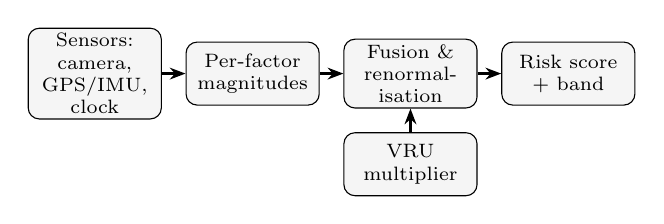
\begin{tikzpicture}[
  node distance=0.3cm,
  box/.style={draw, rounded corners, align=center, text width=1.55cm, minimum height=0.8cm, font=\scriptsize, fill=gray!8, inner sep=2pt},
  arr/.style={-{Stealth[length=2mm]}, thick}
]
\node[box] (sensors) {Sensors: camera, GPS/IMU, clock};
\node[box, right=of sensors] (factors) {Per-factor magnitudes};
\node[box, right=of factors] (fusion) {Fusion \& renormalisation};
\node[box, right=of fusion] (score) {Risk score + band};
\node[box, below=of fusion] (vru) {VRU multiplier};

\draw[arr] (sensors) -- (factors);
\draw[arr] (factors) -- (fusion);
\draw[arr] (fusion) -- (score);
\draw[arr] (vru) -- (fusion);
\end{tikzpicture}
\caption{Data flow through the risk-fusion engine. A missing sensor drops its factor instead of scoring it as safe; the fusion step renormalises the remaining weights, and the reported band's width is exactly the unobserved weight mass.}
\label{fig:architecture}
\end{figure}

\subsection{Observability-aware risk fusion}

Given the available driver, vehicle, road, traffic, perception, and environmental state, the engine computes a magnitude in $[0,1]$ for each factor and fuses them as a weighted sum. The base weights are ordered by each factor's share of Indian road deaths rather than by how easy it is to measure: driver distraction 0.28, speed 0.22, VRU exposure 0.20, road quality 0.13, lane drift 0.09, and traffic congestion 0.08, with a seventh, low-light environmental factor weighted at 0.10 and folded in so that the six perception factors keep their exact relative weights whenever it is absent.

Two design choices do the actual work here. First, a factor with no sensor behind it — no cabin camera, so no distraction signal; no lane markings, so no lane-drift signal — is dropped and its weight is renormalised across the factors that are observed, rather than silently scored as zero, which would read as "safe." This keeps the output a genuine 0--100 score that stays comparable across sensor suites and across the very different road types a vehicle might be on. Second, the point score alone assumes an unmeasured factor behaves like the average of what was measured; a calibrated band makes that assumption explicit, with its lower bound assuming every unmeasured factor is benign and its upper bound assuming the worst, so the band's width is exactly the unobserved weight. A fully instrumented vehicle collapses the band to a point; a speed-only deployment produces roughly a 30-point band (for example, a 28\% point score becomes a 17--54\% band), an honest admission that the system cannot see enough to be more precise.

Because the fusion is additive, the contributing-factor breakdown the system reports is exactly the decomposition of the score, not a post-hoc approximation of one.

\paragraph{Formal statement} Let $F=\{1,\dots,7\}$ index the factors above with fixed base weights $w_i$ and total $W_F = \sum_{i\in F} w_i$ (the seven published weights are rounded to two significant figures and need not sum to exactly 1; the renormalisation below is defined so that this never matters). Let $O \subseteq F$ be the subset actually observed on a given deployment, with observed weight mass $W_O = \sum_{i \in O} w_i$ and unobserved weight mass $W_U = W_F - W_O$. Writing $x_i \in [0,1]$ for the magnitude the engine extracts for factor $i$, the reported point score on a 0--100 scale is the weighted average over only the observed factors,
\begin{equation}
R = 100 \sum_{i \in O} \frac{w_i}{W_O}\, x_i,
\label{eq:fusion-point}
\end{equation}
which reduces to the full seven-factor weighted average whenever $O = F$, and is exactly what results from imputing every unobserved factor with the weighted average of the observed ones. The calibrated band around $R$ instead normalises by the fixed total $W_F$ and does not impute: the lower bound scores every unobserved factor as benign ($x_i = 0$) and the upper bound scores every unobserved factor at its worst ($x_i = 1$),
\begin{equation}
R_{\mathrm{lo}} = 100 \sum_{i \in O} \frac{w_i}{W_F}\, x_i, \qquad
R_{\mathrm{hi}} = R_{\mathrm{lo}} + 100\, \frac{W_U}{W_F},
\label{eq:fusion-band}
\end{equation}
so that the band width $R_{\mathrm{hi}} - R_{\mathrm{lo}} = 100\,W_U/W_F$ is, by construction, exactly the unobserved share of the total weight mass, $R$ always falls inside $[R_{\mathrm{lo}}, R_{\mathrm{hi}}]$, and the band collapses to the single point $R_{\mathrm{lo}}=R=R_{\mathrm{hi}}$ once every sensor is present. Algorithm~\ref{alg:fusion} gives the procedure that computes $(R, R_{\mathrm{lo}}, R_{\mathrm{hi}})$ from whichever sensors happen to be live.

\begin{algorithm}[t]
\caption{Observability-aware risk fusion}
\label{alg:fusion}
\begin{algorithmic}[1]
\Require base weights $\{w_i\}_{i\in F}$ with total $W_F = \sum_{i\in F} w_i$, sensor availability mask $a_i \in \{0,1\}$, raw factor readings
\Ensure point score $R$, band $[R_{\mathrm{lo}}, R_{\mathrm{hi}}]$, factor contributions
\State $O \gets \{ i \in F : a_i = 1 \}$
\State $W_O \gets \sum_{i \in O} w_i$; \ $W_U \gets W_F - W_O$
\For{$i \in O$}
  \State $x_i \gets$ \textsc{ExtractMagnitude}$(i)$ \Comment{clipped to $[0,1]$}
\EndFor
\State $m \gets$ \textsc{VruMultiplier}(helmet, triple-riding counts) \Comment{Eq.~\eqref{eq:vru-mult}}
\State $x_{\mathrm{vru}} \gets \min(m \cdot x_{\mathrm{vru}},\, 1)$ \Comment{if VRU exposure is observed}
\State $R \gets 100 \sum_{i \in O} (w_i / W_O)\, x_i$
\State $R_{\mathrm{lo}} \gets 100 \sum_{i \in O} (w_i / W_F)\, x_i$
\State $R_{\mathrm{hi}} \gets R_{\mathrm{lo}} + 100\,(W_U / W_F)$
\State contributions $\gets \{ (i, 100\, w_i x_i / W_O) : i \in O \}$
\State \Return $R$, $[R_{\mathrm{lo}}, R_{\mathrm{hi}}]$, contributions
\end{algorithmic}
\end{algorithm}

\subsection{VRU-first weighting and per-rider vulnerability}

Two-wheelers and pedestrians are kept as distinct perception classes throughout the pipeline and weighted for exposure, meaning proximity combined with crowding, rather than folded into a generic "other road user" bucket. A fine-tuned YOLOv11 detector further classifies each rider as helmeted, bare-headed, or riding three-up; those counts become a scene-level vulnerability multiplier. Using WHO's estimate that a helmet cuts fatality risk by roughly 42\% \cite{who2006}, a bare head is treated as $1/(1-0.42) \approx 1.72\times$ the risk, triple-riding adds a bounded aggravating factor of about $1.4\times$, and the product of the two is capped at $1.85\times$ so no single scene can dominate the score. Formally, with $b, t \in \{0,1\}$ indicating whether the scene contains at least one bare-headed rider or one triple-riding instance,
\begin{equation}
m(b,t) = \min\!\big(1.72^{\,b} \times 1.4^{\,t},\ 1.85\big),
\label{eq:vru-mult}
\end{equation}
and this multiplier amplifies the VRU-exposure magnitude before weighting, so the score stays additive and the reason it moved stays legible.

\subsection{Predictive black-spot discovery}

The same 500~m unit iRAD uses is instead nominated from near-misses: every vehicle pass through a cell is the exposure denominator, and cells are ranked by a Wilson score lower bound rather than a raw near-miss rate, so a stretch can be flagged before anyone is hurt there, and a cell with one near-miss out of one pass cannot outrank a well-attested one. Formally, for a cell with $k$ near-misses out of $n$ vehicle passes, writing $\hat p = k/n$ and $z = z_{1-\alpha/2}$ for the standard normal quantile,
\begin{equation}
\mathrm{WLB}(k,n) = \frac{\hat p + \dfrac{z^2}{2n} - z\sqrt{\dfrac{\hat p (1-\hat p)}{n} + \dfrac{z^2}{4n^2}}}{1 + \dfrac{z^2}{n}},
\label{eq:wilson}
\end{equation}
and cells are ranked in descending order of $\mathrm{WLB}(k,n)$ rather than $\hat p$ itself, which is what suppresses a single unlucky pass at a low-traffic cell. Algorithm~\ref{alg:blackspot} summarises the nomination procedure end to end.

\begin{algorithm}[t]
\caption{Predictive black-spot nomination}
\label{alg:blackspot}
\begin{algorithmic}[1]
\Require stream of vehicle passes and near-miss events, each geotagged; cell size 500~m; confidence level $1-\alpha$
\Ensure ranked list of nominated cells
\State Partition the road network into 500~m cells $\{c_1, \dots, c_M\}$
\State $n_c \gets 0$, $k_c \gets 0$ for every cell $c$
\For{each vehicle pass or near-miss event $e$}
  \State $c \gets$ cell containing $e$'s location
  \State $n_c \gets n_c + 1$ \Comment{every pass counts toward exposure}
  \If{$e$ is a near-miss, i.e.\ fused risk $R \geq$ threshold}
    \State $k_c \gets k_c + 1$
  \EndIf
\EndFor
\For{each cell $c$ with $n_c > 0$}
  \State score$(c) \gets \mathrm{WLB}(k_c, n_c)$ \Comment{Eq.~\eqref{eq:wilson}}
\EndFor
\State \Return cells sorted by score$(c)$, descending
\end{algorithmic}
\end{algorithm}

\subsection{Environmental context and temporal forecast}

A time-of-day lighting-risk factor is grounded in MoRTH's own published crash-timing data, under which the 18:00--21:00 window holds 20.4\% of all accidents, the single highest three-hour band on record \cite{morth}; because it reads from the clock rather than a camera, it is available on every deployment regardless of hardware. A self-supervised temporal model separately extrapolates each vehicle's own risk trend over time.

\subsection{End-to-end system architecture}
\label{sec:full-architecture}

Fig.~\ref{fig:full-architecture} expands Fig.~\ref{fig:architecture} into the complete pipeline described in this section: three sensor streams feed four perception and estimation models; their outputs become the seven per-factor magnitudes of Eq.~\eqref{eq:fusion-point} and the VRU multiplier of Eq.~\eqref{eq:vru-mult}; the fusion engine of Algorithm~\ref{alg:fusion} combines them under whichever sensor mask is live; and the resulting score and band drive four downstream consumers, one of which, black-spot nomination, is Algorithm~\ref{alg:blackspot} running continuously over the fused engine's own high-risk events. The operator dashboard at the bottom is the same interface captured in Figs.~\ref{fig:screenshot-live} and~\ref{fig:screenshot-blackspots}.

\begin{figure*}[!t]
\centering
\resizebox{\textwidth}{!}{%
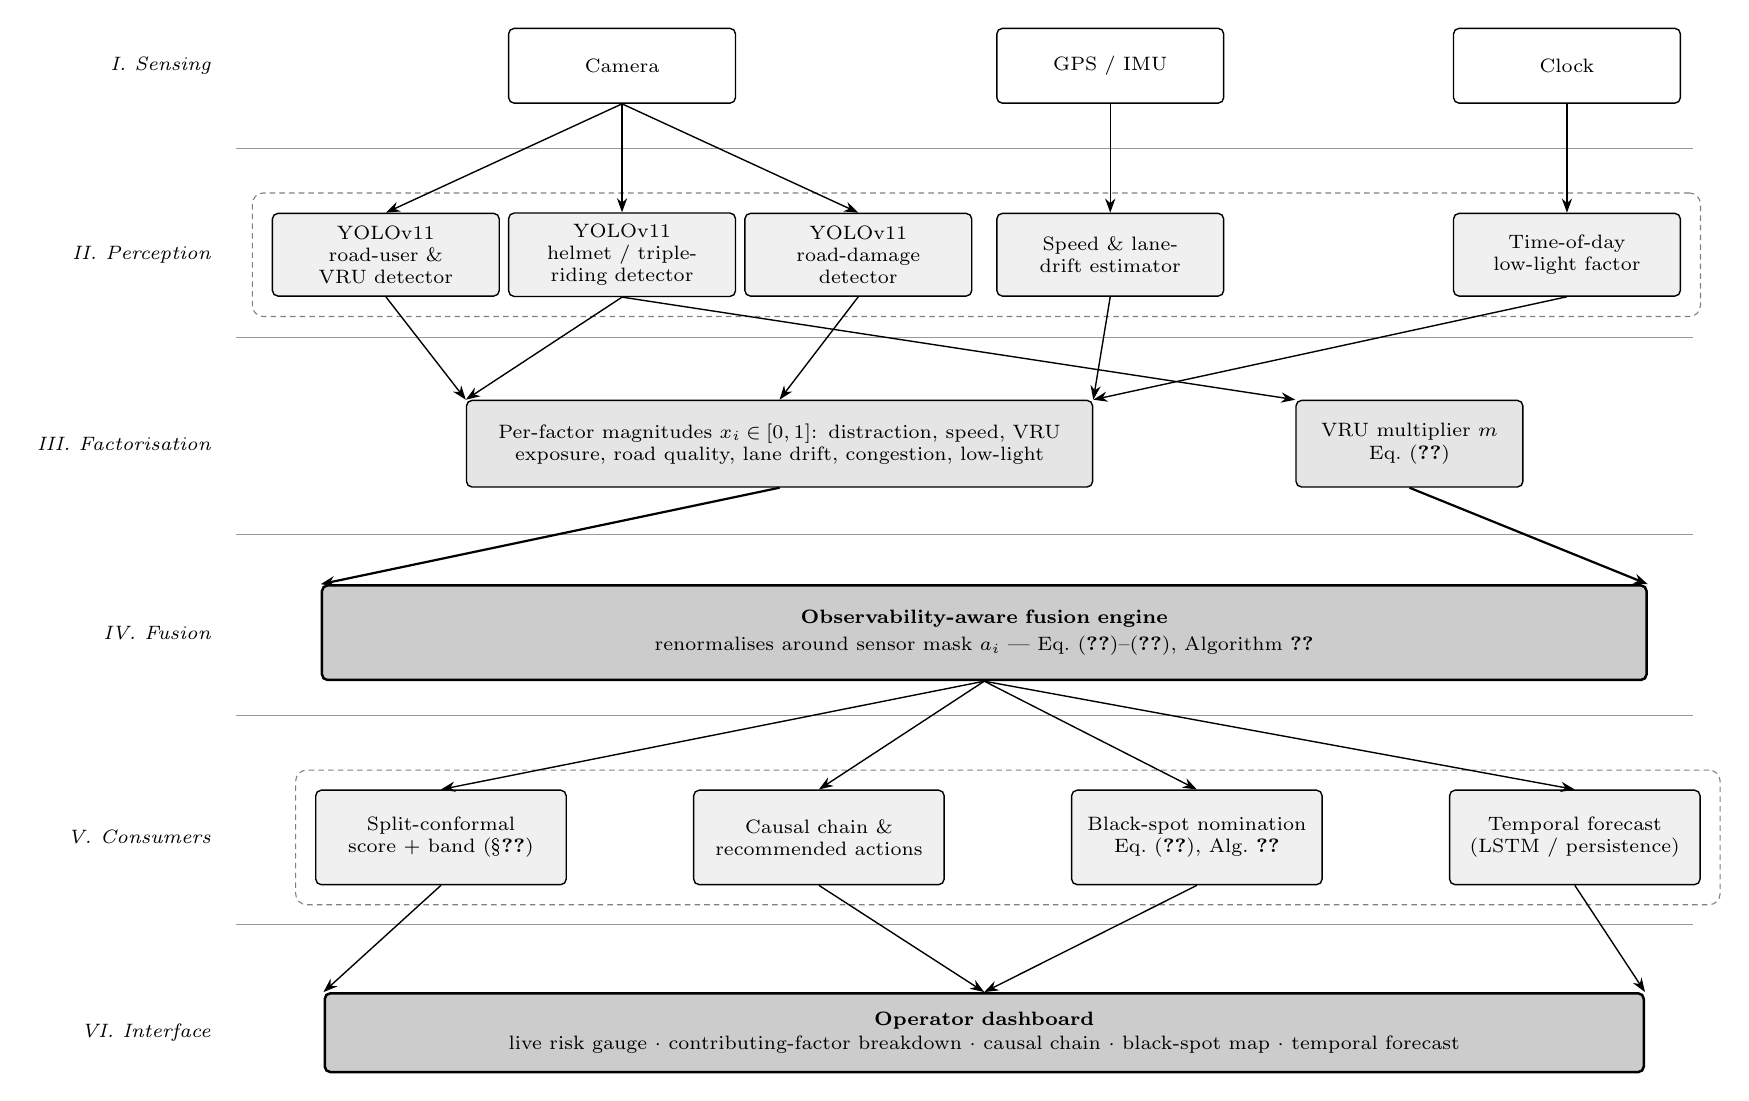
\begin{tikzpicture}[
  sense/.style={draw=black, line width=0.5pt, rounded corners=2pt, align=center, text width=2.6cm, font=\scriptsize, fill=white, inner sep=4pt, minimum height=0.95cm},
  percep/.style={draw=black, line width=0.5pt, rounded corners=2pt, align=center, text width=2.6cm, font=\scriptsize, fill=black!6, inner sep=4pt, minimum height=1.05cm},
  factor/.style={draw=black, line width=0.5pt, rounded corners=2pt, align=center, text width=7.6cm, font=\scriptsize, fill=black!10, inner sep=5pt, minimum height=1.1cm},
  factorsm/.style={draw=black, line width=0.5pt, rounded corners=2pt, align=center, text width=2.6cm, font=\scriptsize, fill=black!10, inner sep=4pt, minimum height=1.1cm},
  core/.style={draw=black, line width=0.9pt, rounded corners=2pt, align=center, text width=16.4cm, font=\scriptsize, fill=black!20, inner sep=6pt, minimum height=1.2cm},
  outp/.style={draw=black, line width=0.5pt, rounded corners=2pt, align=center, text width=2.9cm, font=\scriptsize, fill=black!6, inner sep=4pt, minimum height=1.2cm},
  dashb/.style={draw=black, line width=0.9pt, rounded corners=2pt, align=center, text width=16.4cm, font=\scriptsize, fill=black!20, inner sep=5pt, minimum height=1cm},
  arr/.style={-{Stealth[length=1.8mm, width=1.3mm]}, line width=0.5pt, draw=black},
  carr/.style={-{Stealth[length=1.8mm, width=1.3mm]}, line width=0.8pt, draw=black},
  stagelabel/.style={font=\scriptsize\itshape, text=black, anchor=east},
  sep/.style={draw=black!40, line width=0.3pt},
]

\draw[sep] (-1.6,9.95) -- (16.9,9.95);
\draw[sep] (-1.6,7.55) -- (16.9,7.55);
\draw[sep] (-1.6,5.05) -- (16.9,5.05);
\draw[sep] (-1.6,2.75) -- (16.9,2.75);
\draw[sep] (-1.6,0.1) -- (16.9,0.1);

\node[stagelabel] at (-1.8,11) {I. Sensing};
\node[stagelabel] at (-1.8,8.6) {II. Perception};
\node[stagelabel] at (-1.8,6.2) {III. Factorisation};
\node[stagelabel] at (-1.8,3.8) {IV. Fusion};
\node[stagelabel] at (-1.8,1.2) {V. Consumers};
\node[stagelabel] at (-1.8,-1.28) {VI. Interface};

\node[sense] (camera) at (3.3,11) {Camera};
\node[sense] (gps) at (9.5,11) {GPS / IMU};
\node[sense] (clock) at (15.3,11) {Clock};

\node[percep] (vrudet) at (0.3,8.6) {YOLOv11\\road-user \& VRU detector};
\node[percep] (helmetdet) at (3.3,8.6) {YOLOv11\\helmet / triple-riding detector};
\node[percep] (damagedet) at (6.3,8.6) {YOLOv11\\road-damage detector};
\node[percep] (speedest) at (9.5,8.6) {Speed \& lane-drift estimator};
\node[percep] (lowlight) at (15.3,8.6) {Time-of-day low-light factor};

\begin{pgfonlayer}{background}
\node[draw=black!50, dash pattern=on 2pt off 1.5pt, line width=0.4pt, rounded corners=4pt, fit=(vrudet)(helmetdet)(damagedet)(speedest)(lowlight), inner sep=7pt] (grpA) {};
\end{pgfonlayer}

\node[factor] (factors) at (5.3,6.2) {Per-factor magnitudes $x_i\!\in\![0,1]$: distraction, speed, VRU exposure, road quality, lane drift, congestion, low-light};
\node[factorsm] (vrumult) at (13.3,6.2) {VRU multiplier $m$\\Eq.~\eqref{eq:vru-mult}};

\node[core] (fusion) at (7.9,3.8) {\textbf{Observability-aware fusion engine}\\[2pt]
\normalfont\scriptsize renormalises around sensor mask $a_i$ --- Eq.~\eqref{eq:fusion-point}--\eqref{eq:fusion-band}, Algorithm~\ref{alg:fusion}};

\node[outp] (conformal) at (1,1.2) {Split-conformal\\score + band (\S\ref{sec:ext-validation})};
\node[outp] (causal) at (5.8,1.2) {Causal chain \&\\recommended actions};
\node[outp] (blackspot) at (10.6,1.2) {Black-spot nomination\\Eq.~\eqref{eq:wilson}, Alg.~\ref{alg:blackspot}};
\node[outp] (forecast) at (15.4,1.2) {Temporal forecast\\(LSTM / persistence)};

\begin{pgfonlayer}{background}
\node[draw=black!50, dash pattern=on 2pt off 1.5pt, line width=0.4pt, rounded corners=4pt, fit=(conformal)(causal)(blackspot)(forecast), inner sep=7pt] (grpB) {};
\end{pgfonlayer}

\node[dashb] (dash) at (7.9,-1.28) {\textbf{Operator dashboard}\\[1pt]
\normalfont\scriptsize live risk gauge $\cdot$ contributing-factor breakdown $\cdot$ causal chain $\cdot$ black-spot map $\cdot$ temporal forecast};

\draw[arr] (camera.south) -- (vrudet.north);
\draw[arr] (camera.south) -- (helmetdet.north);
\draw[arr] (camera.south) -- (damagedet.north);
\draw[arr] (gps.south) -- (speedest.north);
\draw[arr] (clock.south) -- (lowlight.north);

\draw[arr] (vrudet.south) -- (factors.north west);
\draw[arr] (damagedet.south) -- (factors.north);
\draw[arr] (speedest.south) -- (factors.north east);
\draw[arr] (lowlight.south) -- (factors.north east);
\draw[arr] (helmetdet.south) -- (factors.north west);
\draw[arr] (helmetdet.south) -- (vrumult.north west);

\draw[carr] (factors.south) -- (fusion.north west);
\draw[carr] (vrumult.south) -- (fusion.north east);

\draw[arr] (fusion.south) -- (conformal.north);
\draw[arr] (fusion.south) -- (causal.north);
\draw[arr] (fusion.south) -- (blackspot.north);
\draw[arr] (fusion.south) -- (forecast.north);

\draw[arr] (conformal.south) -- (dash.north west);
\draw[arr] (causal.south) -- (dash.north);
\draw[arr] (blackspot.south) -- (dash.north);
\draw[arr] (forecast.south) -- (dash.north east);
\end{tikzpicture}%
}
\caption{End-to-end architecture. Raw sensor streams (I) are turned by learned perception and estimation models (II) into per-factor magnitudes and the VRU multiplier (III); the core fusion engine (IV, shaded darker to mark it as the centrepiece) renormalises around whichever sensors are live (Algorithm~\ref{alg:fusion}) and hands its score to four consumers (V), one of which, black-spot nomination, continuously re-runs Algorithm~\ref{alg:blackspot} over the engine's own high-risk events; all four surface in the operator dashboard (VI), shown in Figs.~\ref{fig:screenshot-live}, \ref{fig:screenshot-vehicle}, and~\ref{fig:screenshot-blackspots}. Shading intensity increases with each block's centrality to the pipeline; dashed boundaries mark the two sub-modules referenced individually in the text.}
\label{fig:full-architecture}
\end{figure*}

\section{Experiments and Results}
\label{sec:results}

Fig.~\ref{fig:screenshot-live} shows the deployed Live Risk view described architecturally in Section~\ref{sec:full-architecture}: the fused score and band, the contributing-factor decomposition of Eq.~\eqref{eq:fusion-point}, the causal chain, and the temporal-forecast panel, all on one screen of the open demonstration system at \url{https://trie-dashboard.vercel.app}.

\begin{figure}[t]
\centering
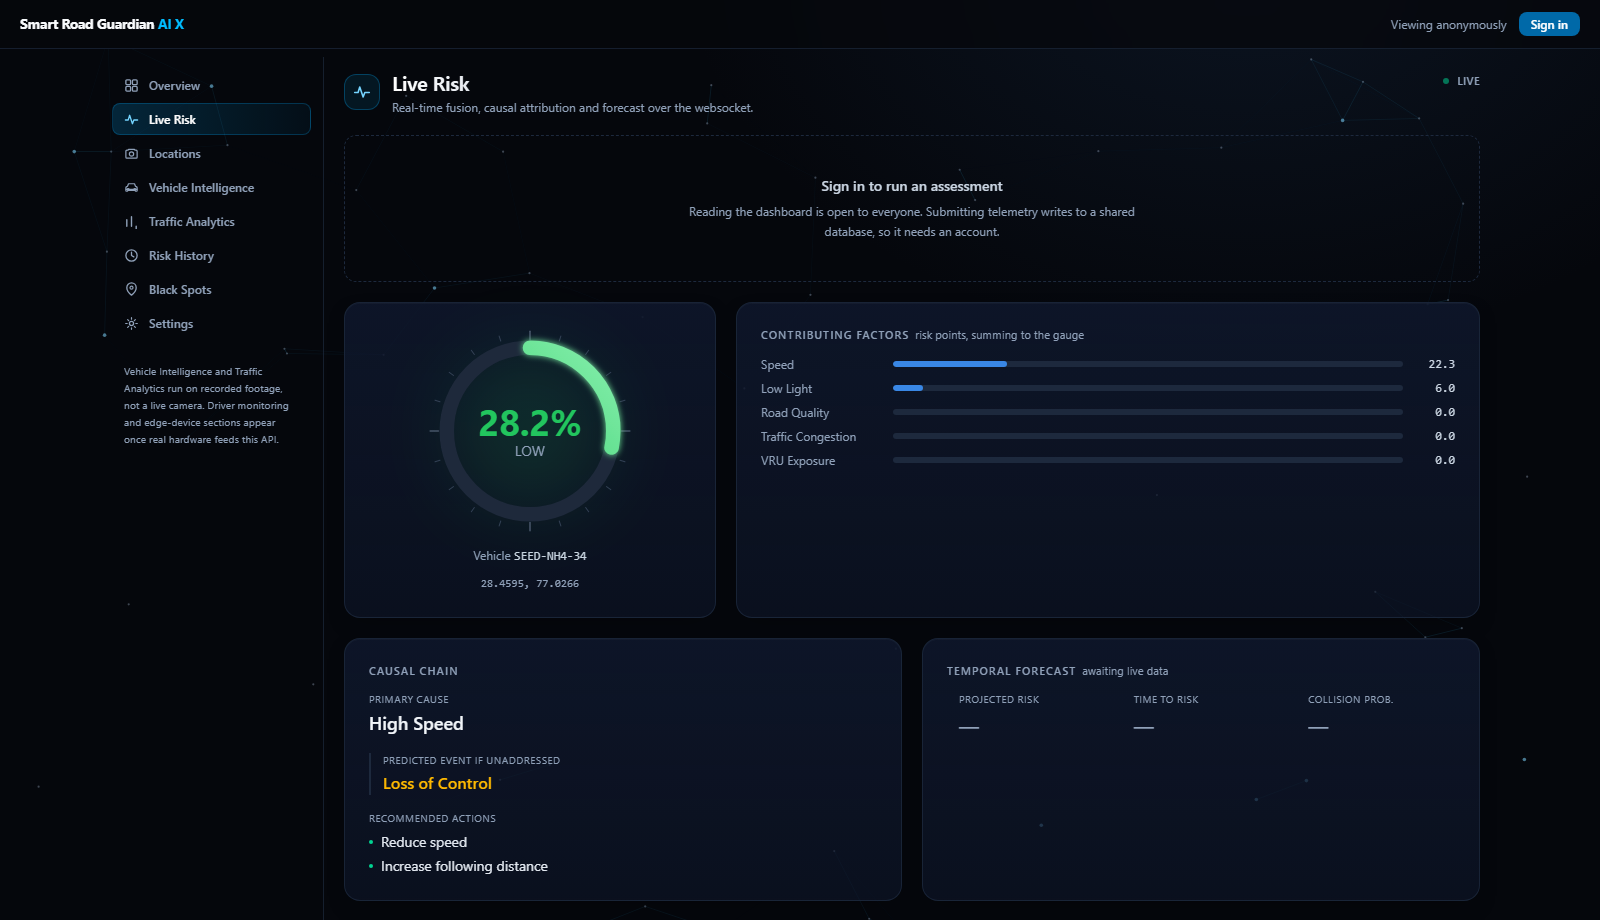
\includegraphics[width=\columnwidth]{figures/screenshot_live_risk.png}
\caption{The deployed Live Risk dashboard: the fused score and band (left), and the additive contributing-factor breakdown, causal chain, and temporal-forecast panel it decomposes into (right), matching Eq.~\eqref{eq:fusion-point} exactly rather than approximating it.}
\label{fig:screenshot-live}
\end{figure}

\subsection{Datasets}
\label{sec:datasets}

Table~\ref{tab:datasets} summarises every dataset used in this paper: one large real-crash source used to validate the factor structure externally, two independent real Indian crash sources used to corroborate it, two Indian imagery sets used to fine-tune the two detectors actually shipped, one Indian imagery set earmarked for a perception fine-tune still in progress (Section~\ref{sec:limitations}), and the government aggregate statistics used for context and cross-checking rather than for fitting any model. One further candidate dataset, a Kaggle release claiming to be Indian road-accident records, was inspected and rejected before use: its road-alignment, location, and vehicle-category fields matched the published Addis Ababa, Ethiopia accident dataset exactly, down to row and column counts, under an incorrect geographic label. We record the rejection rather than silently omitting the dataset, since the check itself is part of the methodology this paper asks a reader to trust.

\begin{table*}[!t]
\centering
\caption{Datasets used in this work}
\label{tab:datasets}
\footnotesize
\setlength{\tabcolsep}{4pt}
\begin{tabular}{p{3.3cm}p{3.1cm}p{3.6cm}p{2.6cm}p{2.3cm}}
\toprule
\multicolumn{1}{c}{\textbf{Dataset}} & \multicolumn{1}{c}{\textbf{Role}} & \multicolumn{1}{c}{\textbf{Scale}} & \multicolumn{1}{c}{\textbf{Geography}} & \multicolumn{1}{c}{\textbf{License}} \\
\midrule
DfT STATS19 \cite{dft2024} & External validation of the factor structure & 128,269 casualty records, 2024 & Great Britain & UK Open Government Licence \\
NHAI highway accident data \cite{khanum2025} & Indian inferential severity model & 4,058 distinct crashes, de-duplicated from 8,116 released rows, 2013--2018 \& 2022--2023 & India, 4 NHAI highway segments & CC-BY-4.0 \\
Media-reported fatal crashes \cite{sharma2025} & Indian descriptive corroboration & 2,898 fatal crashes, 2022--2023 & India, national & CC BY \\
RDD2022, Indian split \cite{arya2024} & Road-damage detector fine-tuning & 1,542 held-out validation images & India & Research use \\
Traffic-violation imagery (Kaggle) & Helmet / triple-riding detector fine-tuning & 11,195 training images & India & Open, attribution \\
India Driving Dataset (IDD) & Perception fine-tune, not yet in production & 15 road-user classes & India & Non-commercial research \\
MoRTH \emph{Road Accidents in India} \cite{morth} & Reference statistics only; not used to fit any model & National annual aggregates, 2021--2024 & India & Government report \\
\bottomrule
\end{tabular}
\end{table*}

\subsection{External validation of the premise on real crashes}
\label{sec:ext-validation}

\paragraph{Data} We use the UK Department for Transport's STATS19 database for 2024 \cite{dft2024}: 100,928 police-reported injury collisions and 128,272 casualties, merged to 128,269 casualty records carrying speed limit, light condition, road-surface condition, and casualty type (vulnerable road user versus vehicle occupant), together with a fatal or non-fatal outcome.

\paragraph{Multivariable logistic regression} With all four factors mutually adjusted, a vulnerable road user carries an odds ratio of 3.66 (95\% CI 3.27--4.09, $p<10^{-115}$) for a fatal outcome; speed limit, per standard deviation, carries 2.23 (2.12--2.34, $p<10^{-229}$); darkness carries 1.73 (1.56--1.92, $p<10^{-24}$); and poor road surface is essentially null, at 1.02 (0.92--1.15, $p=0.67$).

\paragraph{Interactions} A likelihood-ratio test ($\chi^2=39.2$, $df=2$, $p=3\times10^{-9}$) shows the speed-by-VRU interaction is significant (OR 1.34, $p<10^{-9}$): VRU risk compounds with speed, exactly as the VRU-first design predicts. The speed-by-darkness interaction is not significant ($p=0.21$). We note this partly because an earlier raw-rate chart of ours had suggested a widening dark-driving penalty at speed; the formal test demoted that impression, and we rely on the test rather than the chart.

\paragraph{Discrimination and calibration} Five-fold cross-validated ROC-AUC is 0.725 (95\% CI 0.713--0.737); a gradient-boosted baseline reaches only 0.733, so the four factors already carry nearly all the signal a more flexible model can extract. The model is well calibrated, with a Brier score of 0.0121 and an expected calibration error of 0.18\%. A leave-one-out ablation shows dropping speed costs the most discrimination ($\Delta$AUC $-0.13$) and dropping poor surface costs essentially nothing ($-0.00$), consistent with its null odds ratio.

\paragraph{Conformal coverage guarantee} We replace the heuristic uncertainty band with class-conditional, by-label split conformal prediction at $\alpha=0.1$, fitted separately for each sensor regime on a three-way split of the 128k casualties. Formally, for a calibration set $\{(x_j, y_j)\}_{j=1}^{n}$ held out within a given sensor regime and class $y \in \{\mathrm{fatal}, \mathrm{non\text{-}fatal}\}$, let $s(x,y) = 1 - \hat f(x)_y$ be the nonconformity score of the fitted model $\hat f$ and let $\hat q_y$ be the $\lceil (n_y+1)(1-\alpha) \rceil / n_y$ empirical quantile of $\{s(x_j, y) : y_j = y\}$. The prediction set
\begin{equation}
C(x) = \{\, y : s(x,y) \leq \hat q_y \,\}
\label{eq:conformal-set}
\end{equation}
then satisfies the distribution-free, class-conditional guarantee $\Pr\big(y \in C(x)\big) \geq 1-\alpha$ for each class $y$, so "cannot rule out fatal" is precisely $\mathrm{fatal} \in C(x)$. The resulting guarantee, that at least 90\% of truly fatal outcomes fall inside the model's "cannot rule out fatal" set, is a guarantee on coverage in expectation over the calibration draw. It is met empirically in every regime on the split we report: 92.8\% with the full sensor suite, 96.5\% with the camera removed, and 94.8\% telemetry-only. Because the fatal class is rare, a single split's empirical coverage carries real sampling noise, roughly $\pm2$ points on about 300 fatal test cases; an independent re-run of the identical code landed at 89.5\%, 95.5\%, and 93.0\% on those same three regimes. A value a point or two under the 90\% target on any one split is therefore consistent with the guarantee rather than a violation of it, and our own automated check accordingly asserts coverage within about two standard errors of target rather than a hard inequality. The cost of the guarantee is the alarm rate, and it is exactly the observability thesis made rigorous: with the full sensor suite the model can confidently clear 32\% of cases of any fatal risk at all, against only 12--17\% once the camera is removed, the same guaranteed fatal recall at a quantified price for fewer sensors, where the model previously shipped only a heuristic band. Fig.~\ref{fig:conformal} plots both runs' empirical coverage against the 90\% target and the corresponding alarm-rate cost side by side. This result is reproducible with \texttt{python -m ai.trie.conformal\_validation}.

\begin{figure}[t]
\centering
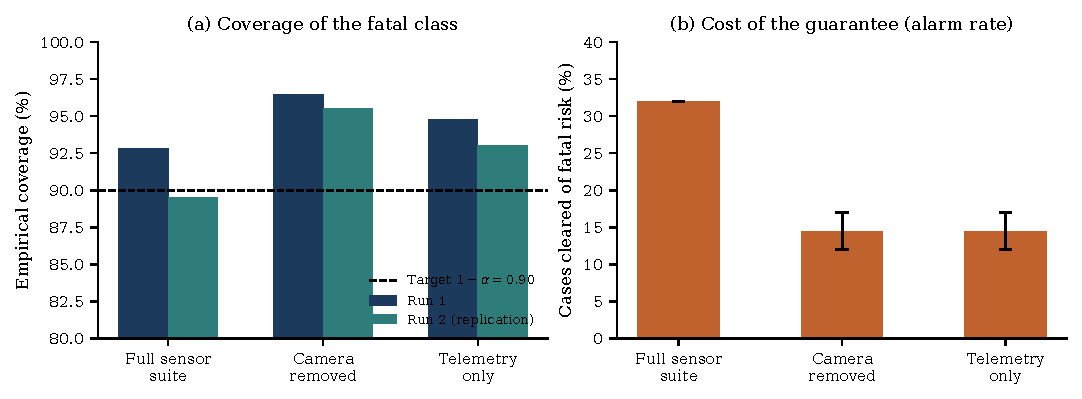
\includegraphics[width=\columnwidth]{figures/fig_conformal_coverage.pdf}
\caption{Class-conditional split-conformal coverage of the fatal class across sensor regimes, for the reported run and an independent replication (a), against the cost of the guarantee in cases the model can confidently clear of fatal risk (b). Coverage tracks the 90\% target in every regime within sampling noise, and the alarm-rate cost falls sharply once the camera is lost, which is the observability thesis made quantitative.}
\label{fig:conformal}
\end{figure}

\paragraph{Interpretation and scope} This experiment validates the factor structure the model rests on — the right factors, in the right direction, in the right order of importance — on real crash records. It is British, not Indian, data: the two VRU classes that dominate Indian deaths, pedestrians and motorcyclists, are exactly the high-fatality classes here too, but Britain's comparatively well-protected cyclists score low, which is an honest cross-domain difference rather than something to paper over. Crash severity is also not identical to the live risk score the system reports day to day. These results are reproducible with \texttt{python -m ai.trie.external\_validation} and \texttt{python -m ai.trie.statistical\_validation}.

\paragraph{Indian corroboration} The British-data caveat above is answered directly with real Indian crashes: 2,898 fatal crashes reported nationally in 2022--2023, extracted by natural-language processing from Times of India coverage \cite{sharma2025}. Vulnerable road users are 56.2\% of the fatal-crash victims in this sample (38.8\% two-wheeler riders, 16.0\% pedestrians, 1.3\% cyclists), consistent in direction with MoRTH's own 66.8\% figure, and 69.5\% of VRU victims were killed by a heavier road user, which is direct support for the exposure argument the VRU-first weighting is built on. Because this is a media-reported, fatal-only sample, it corroborates the premise descriptively rather than re-fitting the severity model, and is reproducible with \texttt{python -m ai.trie.india\_validation}.

\paragraph{Indian inferential model} To remove the fatal-only limitation, we use a second Indian source that does carry non-fatal crashes: 4,058 distinct record-level crashes from National Highways Authority of India highway segments, dated 2013--2018 and 2022--2023, with no records for 2019--2021 \cite{khanum2025}, decoded with the authors' own published codebook. The released file lists every crash twice, 8,116 rows for those 4,058 crashes, with 4,054 of the 4,058 rows identical across the two halves; we detect and remove the duplicate, since treating it as independent would narrow the confidence intervals by roughly $\sqrt{2}$ and leak duplicate rows across cross-validation folds. A multivariable logistic regression on a killed-or-seriously-injured outcome, the direct Indian counterpart to the STATS19 model above, supports the same factor structure: VRU involvement carries an odds ratio of 1.97 (95\% CI 1.73--2.26, $p\approx3\times10^{-23}$); a VRU struck by a heavier vehicle carries 1.48 (1.07--2.05, $p=0.018$); overspeeding carries 1.23 (1.09--1.40, $p=0.001$); and night-time carries 1.25 (1.10--1.42, $p<10^{-3}$). A crash involving a vulnerable road user very nearly doubles the adjusted odds of a severe outcome, and dropping VRU involvement from the model costs more discrimination than dropping any other factor. Discrimination here is modest, and we report it as such: cross-validated AUC is 0.58 (95\% CI 0.56--0.60), no better than a gradient-boosted baseline at 0.57. We also report, in full, that sharp curves come out protective (odds ratio 0.46, $p=0.004$), a known highway-exposure and behavioural-compensation artefact, while the undivided-road (0.84) and adverse-weather (0.88) terms point the same way but are not statistically significant ($p\approx0.09$). The scope of this result is NHAI national highways specifically, a high-speed inter-urban profile rather than urban Indian roads generally; the outcome is injury severity, not the live risk score; and night-time is an 18:00--06:00 proxy, since the data carries no measured light-condition field. Within that scope, this is an inferential confirmation of the VRU-first factor structure on real Indian crashes, modest where discrimination is concerned but consistent in direction and significance on the factor that matters most to the thesis. Reproducible with \texttt{python -m ai.trie.india\_severity\_model}.

Fig.~\ref{fig:forest} summarises both multivariable models as forest plots of adjusted odds ratios: the VRU-related terms sit well clear of unity with tight confidence intervals in both the British and the Indian model, while the factors that do not survive adjustment, poor road surface in STATS19 and the sharp-curve, undivided-road, and weather terms in NHAI, are shown with the same visual weight rather than quietly omitted.

\begin{figure}[t]
\centering
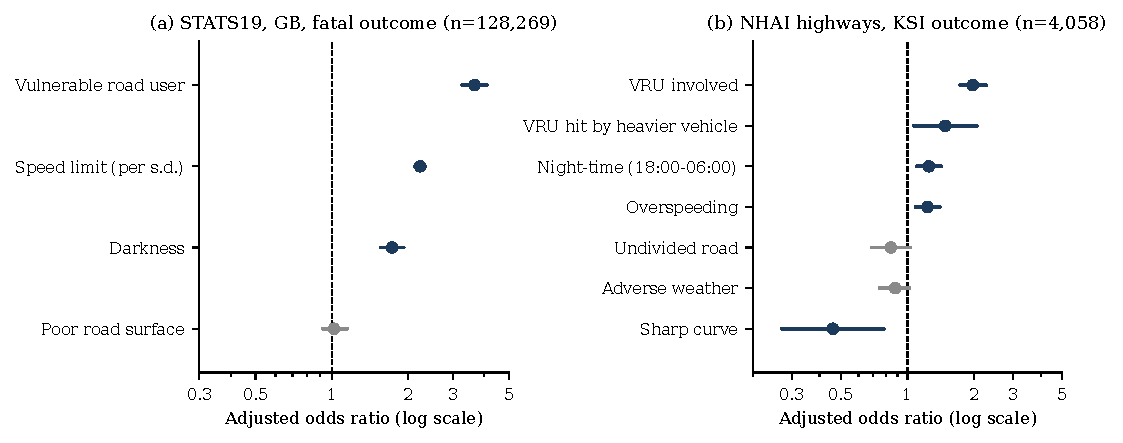
\includegraphics[width=\columnwidth]{figures/fig_forest_odds_ratios.pdf}
\caption{Adjusted odds ratios (95\% CI, log scale) for a fatal outcome in STATS19 (a) and a killed-or-seriously-injured outcome on NHAI highways (b). Grey whiskers cross the line of no effect (OR = 1); navy whiskers do not. VRU involvement is the largest, most consistent effect in both real-crash datasets.}
\label{fig:forest}
\end{figure}

Fig.~\ref{fig:auc}(a) places every ROC-AUC reported against real crash records on one axis, with 95\% confidence intervals where we report them, so the modest NHAI discrimination and the markedly stronger black-spot precursor and STATS19 figures are read off a common scale rather than compared across separate paragraphs.

\begin{figure}[t]
\centering
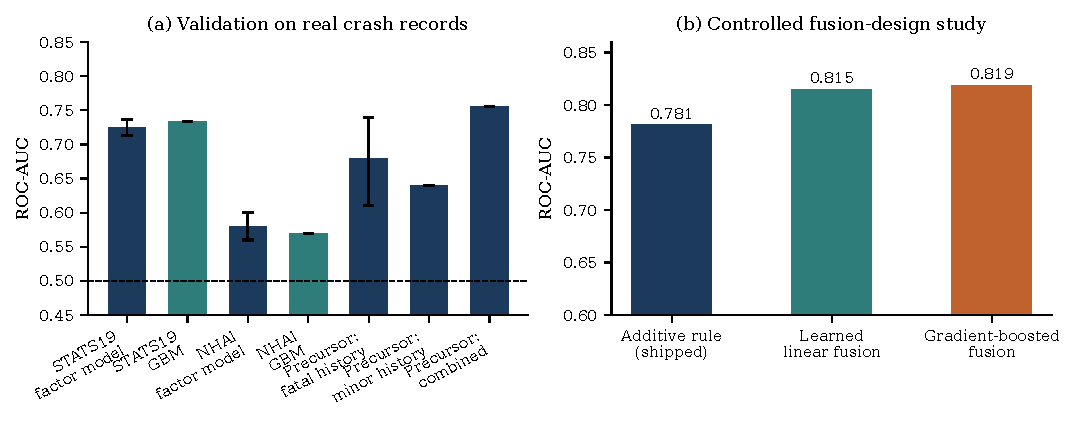
\includegraphics[width=\columnwidth]{figures/fig_auc_comparison.pdf}
\caption{Discrimination (ROC-AUC) across every experiment validated on real crash or precursor data (a), and across the controlled fusion-design study of Section~\ref{sec:fusion-results} (b). Error bars are 95\% confidence intervals where reported.}
\label{fig:auc}
\end{figure}

\subsection{Per-rider vulnerability detector}
\label{sec:rider-detector}

A YOLOv11s detector, fine-tuned for helmet, no-helmet, triple-riding, and plate classes on 11,195 training images at 640px resolution (batch size 12), evaluated on 383 held-out images after training to 25 epochs with the best checkpoint at epoch 15, reaches an overall mAP@50 of 78.2\%. Per class, triple-riding reaches 91.0, plate 83.2, no-helmet 75.6, and with-helmet 62.9, the noisiest class with only 27 validation instances. We present this as a component metric feeding the vulnerability multiplier above, not as a leaderboard claim. Reproducible with \texttt{python -m ai.training.train\_helmet \mbox{-{}-evaluate}}.

Fig.~\ref{fig:screenshot-vehicle} shows the same detector running frame-by-frame on recorded Indian street footage in the deployed Vehicle Intelligence view, with the resulting multiplier of Eq.~\eqref{eq:vru-mult} reported live alongside the detections it is computed from.

\begin{figure}[t]
\centering
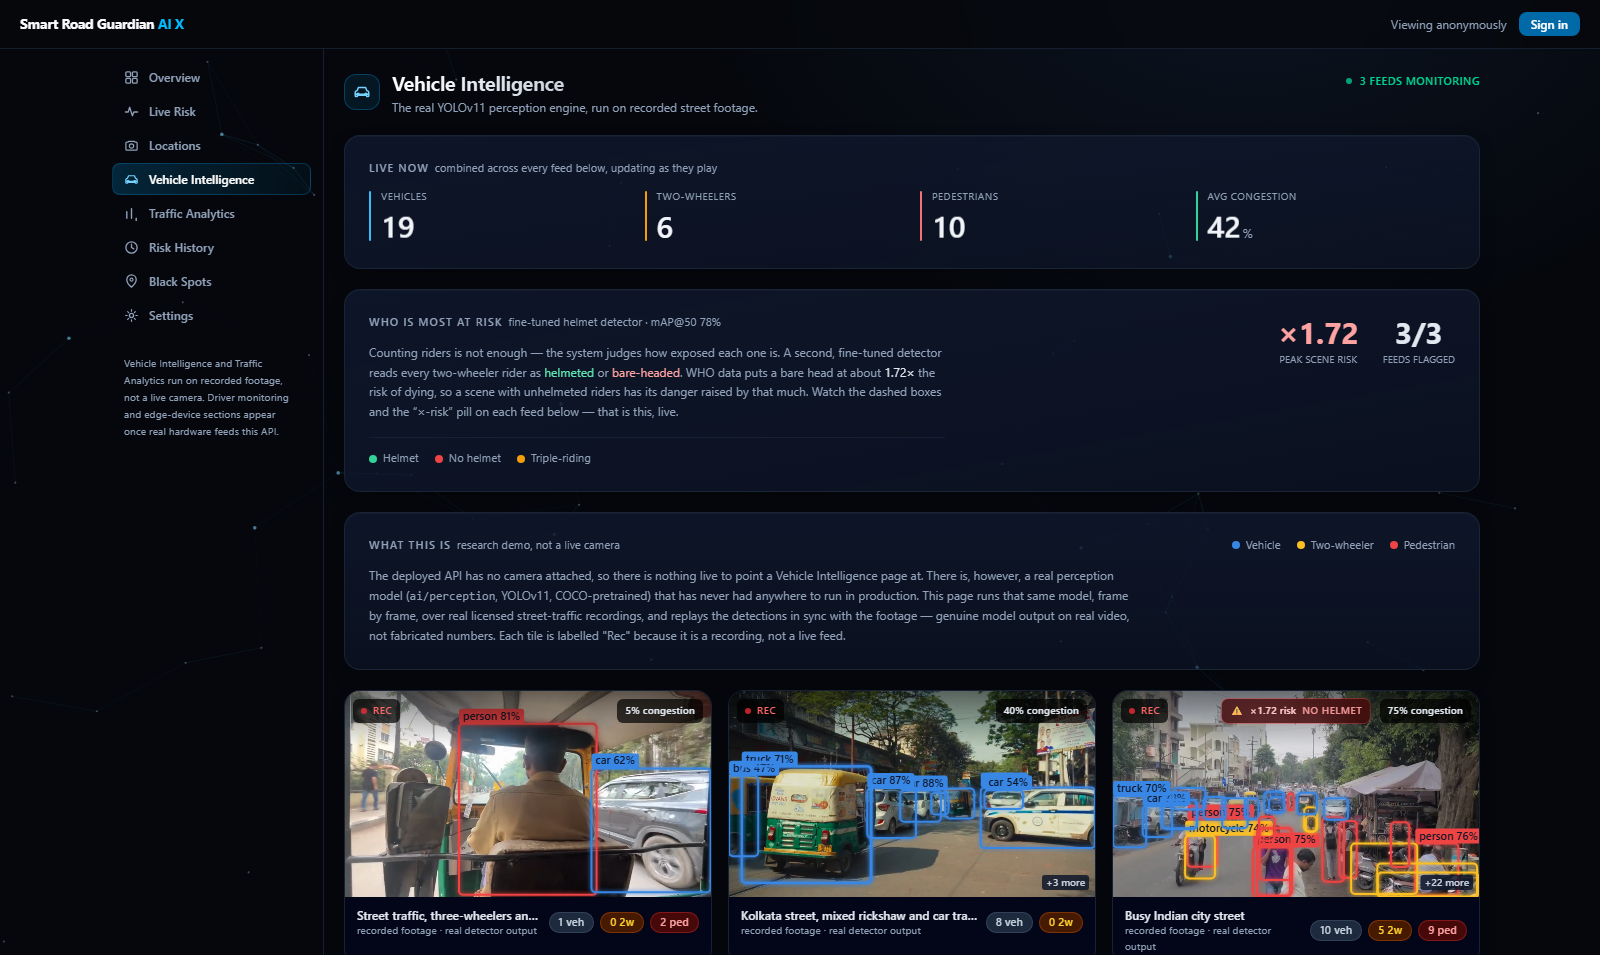
\includegraphics[width=\columnwidth]{figures/screenshot_vehicle_intel.png}
\caption{The deployed Vehicle Intelligence view: the fine-tuned YOLOv11 detector running on recorded Indian street footage, with per-rider helmet/no-helmet/triple-riding boxes and the resulting scene-level multiplier $m$ (Eq.~\eqref{eq:vru-mult}) reported top right.}
\label{fig:screenshot-vehicle}
\end{figure}

\subsection{Predictive black-spot discovery: evaluation}
\label{sec:blackspot-results}

\paragraph{Controlled evaluation} Across 40 random seeds and two traffic volumes, comparing a genuinely dangerous stretch against a busy-but-safe one, the engine achieves 100\% detection and 0\% false positives on the busy-but-safe road, which is the load-bearing result here: it shows the system is flagging danger rather than merely traffic volume. Median lead time over iRAD's own reactive threshold is one day on the busy stretch and 7.5 days on the quiet one, against iRAD's own 170 to 888 days, or never, within its three-year window. We are explicit that this is a controlled evaluation against authored ground truth, and that a true field retrospective against MoRTH's published black-spot list needs near-miss telemetry for real Indian locations, which is not publicly available. Reproducible with \texttt{python -m ai.blackspot.evaluate}.

Fig.~\ref{fig:screenshot-blackspots} shows the deployed Black-Spot Intelligence view the engine of Algorithm~\ref{alg:blackspot} renders this evaluation into: nominated stretches sized by near-miss count and coloured by the countermeasure category, which is the same 500~m unit and Wilson-ranked output iRAD's own reactive criterion is compared against above.

\begin{figure}[t]
\centering
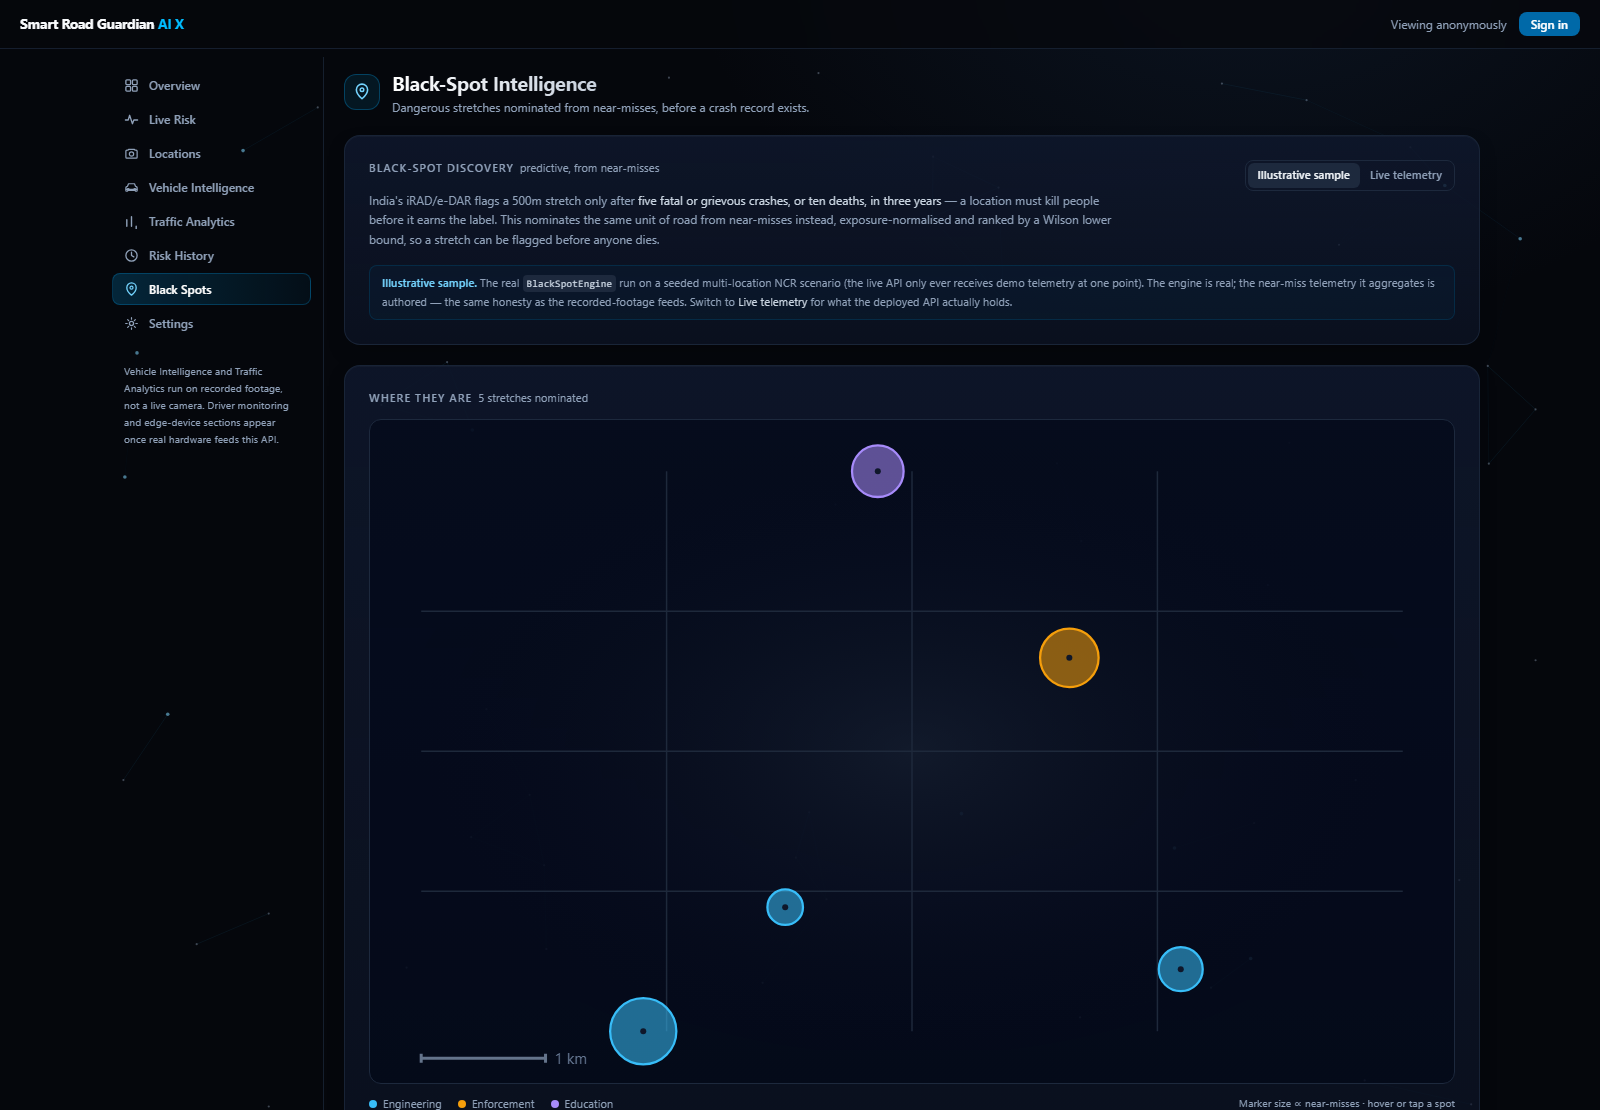
\includegraphics[width=\columnwidth]{figures/screenshot_blackspots.png}
\caption{The deployed Black-Spot Intelligence view: five stretches nominated from near-misses (Algorithm~\ref{alg:blackspot}), marker size proportional to near-miss count and colour indicating the recommended engineering, enforcement, or education response.}
\label{fig:screenshot-blackspots}
\end{figure}

\paragraph{A negative retrospective result on real crashes} Field validation against MoRTH's black spots needs near-miss telemetry that nobody publishes, but real crash data does permit a test of the hypothesis underneath predictive discovery: that lower-severity crashes at a stretch anticipate the severe ones before iRAD's own rule would catch them. Using the de-duplicated NHAI records above, we build 831 real 500~m cells across three inferred road segments, of which 94 meet iRAD's own rule of five or more fatal or grievous crashes within three years. The design, including a permutation-based null, was fixed in advance. A precursor rule requiring three or more minor or non-injury crashes within a trailing year fires before iRAD qualification in 52\% of the 94 qualifying cells, a median of 329 days ahead; but a severity-permutation null, which shuffles severities among the same crashes within each road while holding places and dates fixed, gives 51\% and 276 days ($p=0.41$; thresholds of two and four crashes give $p\geq0.47$), which indicates the apparent lead time is a crash-volume effect rather than a severity effect. On the prediction side, splitting each road at its median crash date, a cell's earlier fatal-or-grievous count predicts two or more such crashes later with an AUC of 0.68 (95\% CI 0.61--0.74); earlier minor crashes alone reach 0.64; total crash volume reaches 0.69. A road-adjusted logistic model using both fatal history and minor-crash history reaches an AUC of 0.755, but the identical model with the minor-crash term removed also reaches 0.755, so the minor crashes' own contribution beyond fatal history and road identity is an AUC difference of 0.000 (95\% CI $-0.005$ to $+0.005$), and their Poisson rate ratio given fatal-crash history is 1.04 (95\% CI 0.99--1.09, $p=0.10$). An earlier version of this comparison, run against road-blind scores rather than a road-adjusted baseline, appeared to favour the combined model; adding the road-adjusted control showed that apparent gain was entirely road-level base rates, not the minor-crash signal, and we report this corrected analysis, superseding our earlier, upward-biased comparison. We therefore find no evidence, on real Indian crash records, that lower-severity crashes carry predictive information beyond a stretch's own severe-crash history and traffic volume. This is not a test of near-miss telemetry, which is a richer and far more frequent signal than recorded minor crashes and is what the deployed engine actually consumes, and that question remains untested; three inferred road segments and 227 positive cells also limit the statistical power available to detect a smaller effect. Reproducible with \texttt{python -m ai.trie.blackspot\_crash\_validation}.

\subsection{Learned fusion and interaction analysis}
\label{sec:fusion-results}

On a controlled ground truth where risk genuinely compounds across factors, a learned fusion model outperforms the hand-set additive rule (ROC-AUC 0.781 for the rule, 0.815 for a linear learned model, and 0.819 for a gradient-boosted model, all calibrated, with Brier scores around 0.16). Friedman's H-statistic applied to the gradient-boosted model recovers the three interactions the rule-based system was authored to encode among its top three by strength: speed-by-road at 0.25, speed-by-VRU at 0.22, and distraction-by-VRU at 0.19. The transparent rule is what ships; the learned model is evidence that the same architecture admits a learned, calibrated fusion when labelled telemetry becomes available. We use the H-statistic rather than SHAP deliberately, since the shipped model is already exactly additive and needs no post-hoc attribution. Reproducible with \texttt{python -m ai.trie.fusion\_study} and \texttt{python -m ai.trie.interaction\_analysis}. Fig.~\ref{fig:auc}(b) plots the three ROC-AUC figures side by side against the accuracy-versus-interpretability trade-off discussed in Section~\ref{sec:discussion}.

\subsection{Supporting components}

A YOLOv11s road-damage detector, fine-tuned for 55 epochs at 640px resolution on the Indian split of RDD2022 \cite{arya2024}, is evaluated on 1,542 held-out images (Table~\ref{tab:damage}). Overall mAP@50 is 33.0\% (mAP@50--95: 14.2\%); we present this as a working component, not a state-of-the-art result, and report the weakest class rather than only the strongest two. Alligator cracks and potholes, the damage types most relevant to vehicle-level risk, are detected reasonably well (57.7\% and 44.3\% mAP@50); transverse cracks are close to non-functional at 1.9\% mAP@50, almost certainly a thin, low-instance-count class that would need more data or class-balancing before being relied on, and we disclose it rather than folding it into the aggregate.

\begin{table}[h]
\centering
\caption{Road-damage detector, per class}
\label{tab:damage}
\small
\begin{tabular}{lrr}
\toprule
\textbf{Class} & \textbf{mAP@50} & \textbf{mAP@50--95} \\
\midrule
Alligator crack & 57.7\% & 27.3\% \\
Pothole & 44.3\% & 16.5\% \\
Longitudinal crack & 28.0\% & 12.5\% \\
Transverse crack & 1.9\% & 0.4\% \\
\midrule
\textbf{Overall} & \textbf{33.0\%} & \textbf{14.2\%} \\
\bottomrule
\end{tabular}
\end{table} On the temporal-forecast side, we found, somewhat to our own surprise, that the linear extrapolation currently shipped (mean absolute error 19.0) is actually worse than simple persistence (13.4), while a small LSTM model (10.1) cuts error by roughly 47\% relative to the shipped approach, a finding we report against ourselves rather than only against a weaker baseline.

\section{Discussion}
\label{sec:discussion}

The result this paper is built around is Section~\ref{sec:ext-validation}: the model's premise is not asserted from authored scenarios but demonstrated on six figures' worth of real crashes, with statistical significance, calibration, and an ablation behind it. The system-level inversions we set out to make are each defended against the prior art surveyed in Section~\ref{sec:related}: predictive instead of reactive, VRU-first rather than occupant-centric, observability-aware instead of silently confident, and explainable by construction rather than by post-hoc attribution. We would also argue that the honesty running through this work is itself part of the contribution: dropping unmeasured factors instead of guessing them, reporting an uncertainty band instead of a false point estimate, demoting an interaction effect the eye initially over-read, and publishing a negative result rather than quietly dropping the experiment that produced it.

A further trade-off worth stating explicitly is interpretability against ceiling accuracy. Section~\ref{sec:fusion-results} shows a learned, gradient-boosted fusion model reaching a materially higher ROC-AUC (0.819) than the transparent additive rule it is compared against (0.781) on the same controlled ground truth. We ship the rule anyway: every factor contribution it reports is the literal arithmetic behind the score rather than a post-hoc approximation of one, and an operator reading an alert, not a researcher reading a paper, is the system's actual audience. The learned variant remains an upgrade path for whenever labelled Indian telemetry exists to train and calibrate it responsibly, rather than something shipped on data it was never validated against.

A second trade-off is geographic transfer. The factor structure validated in Section~\ref{sec:ext-validation} and corroborated on Indian data immediately after it transfers in direction, and for several factors in relative order of importance; it does not necessarily transfer in magnitude. Britain's protected-cyclist environment suppresses a fatality channel that is far more exposed on an Indian road, and neither Indian crash source used here carries the labelled live-telemetry factors the deployed fusion engine actually consumes. The Indian results in this paper therefore validate the premise behind the system rather than its live risk score directly, a distinction Section~\ref{sec:limitations} returns to.

\section{Limitations and Future Work}
\label{sec:limitations}

The headline predictive-discovery claim remains simulation-only. The highest-value next experiment is a field retrospective against MoRTH's own black-spot list, which requires near-miss telemetry for real Indian locations, meaning a data partnership with traffic police, a city, or iRAD itself, not a modelling change on our end. External validation of the factor structure, similarly, is British rather than Indian data; the factor structure appears to transfer, but the magnitudes and the India-specific vehicle mix, auto-rickshaws and six-up motorcycles among them, likely do not, and an Indian labelled crash-feature dataset is the asset that would let us check. Perception itself is presently a COCO-pretrained baseline for general road users, with the fine-tuned helmet detector as the one exception; we make no leaderboard claim there and none is needed for the argument this paper makes. Finally, the learned fusion model described in Section~\ref{sec:fusion-results} is not what ships; it waits on labelled Indian telemetry that does not yet exist, and the transparent rule-based model remains what runs in production.

\section{Conclusion}

Road safety for the roads India actually has needs a system that acts before the crash, protects the people most exposed to it, and is honest about what it cannot see. We have presented one, and, we believe unusually for a project of this kind, shown that the factor relationships it rests on hold up on real crash records rather than only on scenarios we authored ourselves. The gap that remains is real Indian field data for the predictive black-spot claim specifically, and we have named that as the next experiment throughout this paper rather than quietly working around it.

\appendix
\section{Reproducibility}

Every quantitative result in this paper is one command away in the open-source repository (Table~\ref{tab:repro}).

\begin{table}[h]
\centering
\caption{Reproducing every result}
\label{tab:repro}
\small
\begin{tabular}{p{4.3cm}p{3.7cm}}
\toprule
\textbf{Result} & \textbf{Command} \\
\midrule
External validation (real crashes) & \texttt{ai.\allowbreak trie.\allowbreak external\_validation} \\
Statistical validation (ORs, interactions, calibration) & \texttt{ai.\allowbreak trie.\allowbreak statistical\_validation} \\
Conformal coverage guarantee & \texttt{ai.\allowbreak trie.\allowbreak conformal\_validation} \\
Indian corroboration (2,898 fatal crashes) & \texttt{ai.\allowbreak trie.\allowbreak india\_validation} \\
Indian inferential severity model (4,058 crashes) & \texttt{ai.\allowbreak trie.\allowbreak india\_severity\_model} \\
Black-spot precursor test (negative result) & \texttt{ai.\allowbreak trie.\allowbreak blackspot\_crash\_validation} \\
Black-spot discovery evaluation & \texttt{ai.\allowbreak blackspot.\allowbreak evaluate} \\
Learned-fusion study & \texttt{ai.\allowbreak trie.\allowbreak fusion\_study} \\
Interaction analysis (H-statistic) & \texttt{ai.\allowbreak trie.\allowbreak interaction\_analysis} \\
Temporal forecast study & \texttt{ai.\allowbreak temporal\_prediction.\allowbreak forecast\_study} \\
Helmet detector evaluation & \texttt{ai.\allowbreak training.\allowbreak train\_helmet \mbox{-{}-evaluate}} \\
Road-damage detector evaluation & \texttt{ai.\allowbreak training.\allowbreak train\_road\_damage \mbox{-{}-evaluate}} \\
\bottomrule
\end{tabular}
\end{table}

Every command above is prefixed with \texttt{python -m} and is run from the repository root; each one downloads or regenerates its own public source data rather than relying on a vendored copy.

\section*{Acknowledgment}
This work received no external funding.

\begin{thebibliography}{37}

\bibitem{morth} Ministry of Road Transport \& Highways, Government of India, \emph{Road Accidents in India}, annual reports, 2021--2024.

\bibitem{gettman2008} D. Gettman, L. Pu, T. Sayed, and S. Shelby, \emph{Surrogate Safety Assessment Model and Validation: Final Report}, Federal Highway Administration, Rep. FHWA-HRT-08-051, 2008.

\bibitem{johnsson2018} C. Johnsson, A. Laureshyn, and T. De Ceunynck, ``In search of surrogate safety indicators for vulnerable road users: a review of surrogate safety indicators,'' \emph{Transp. Rev.}, vol. 38, no. 6, pp. 765--785, 2018, doi: 10.1080/01441647.2018.1442888.

\bibitem{hauer2002} E. Hauer, D. W. Harwood, F. M. Council, and M. S. Griffith, ``Estimating safety by the empirical Bayes method: a tutorial,'' \emph{Transp. Res. Rec.}, vol. 1784, pp. 126--131, 2002, doi: 10.3141/1784-16.

\bibitem{aashto2010} American Association of State Highway and Transportation Officials, \emph{Highway Safety Manual}, 1st ed. Washington, DC, USA: AASHTO, 2010.

\bibitem{cheng2005} W. Cheng and S. P. Washington, ``Experimental evaluation of hotspot identification methods,'' \emph{Accid. Anal. Prev.}, vol. 37, no. 5, pp. 870--881, 2005, doi: 10.1016/j.aap.2005.04.015.

\bibitem{chang2022} I. Chang, H. Park, E. Hong, J. Lee, and N. Kwon, ``Predicting effects of built environment on fatal pedestrian accidents at location-specific level: application of XGBoost and SHAP,'' \emph{Accid. Anal. Prev.}, vol. 166, 2022, Art. no. 106545.

\bibitem{who2006} World Health Organization, \emph{Helmets: A Road Safety Manual for Decision-Makers and Practitioners}. Geneva, Switzerland: WHO, 2006, ISBN 978-92-4-156299-7 (2nd ed., 2023).

\bibitem{jia2021} W. Jia, S. Xu, Z. Liang, Y. Zhao, H. Min, S. Li, and Y. Yu, ``Real-time automatic helmet detection of motorcyclists in urban traffic using improved YOLOv5 detector,'' \emph{IET Image Process.}, vol. 15, no. 14, pp. 3623--3637, 2021, doi: 10.1049/ipr2.12295.

\bibitem{agorku2023} G. Agorku, D. Agbobli, V. Chowdhury, K. Amankwah-Nkyi, A. Ogungbire, P. A. Lartey, and A. Aboah, ``Real-time helmet violation detection using YOLOv5 and ensemble learning,'' arXiv:2304.09246, 2023.

\bibitem{vovk2022} V. Vovk, A. Gammerman, and G. Shafer, \emph{Algorithmic Learning in a Random World}, 2nd ed. Cham, Switzerland: Springer, 2022.

\bibitem{angelopoulos2023} A. N. Angelopoulos and S. Bates, ``A gentle introduction to conformal prediction and distribution-free uncertainty quantification,'' \emph{Found. Trends Mach. Learn.}, vol. 16, no. 4, pp. 494--591, 2023, doi: 10.1561/2200000101.

\bibitem{romano2020} Y. Romano, M. Sesia, and E. J. Cand\`es, ``Classification with valid and adaptive coverage,'' in \emph{Advances in Neural Information Processing Systems (NeurIPS)}, vol. 33, 2020.

\bibitem{who2023} World Health Organization, \emph{Global Status Report on Road Safety 2023}. Geneva, Switzerland: WHO, 2023, ISBN 978-92-4-008651-7.

\bibitem{fhwa2022vru} Federal Highway Administration, \emph{Ensuring Cooperative Driving Automation (CDA) and Vulnerable Road Users (VRUs) Safety Through Infrastructure}, Rep. FHWA-HRT-22-085, 2022, doi: 10.21949/1521914.

\bibitem{erso2024} European Commission, Directorate-General for Mobility and Transport, \emph{European Road Safety Observatory: Thematic Reports on Vulnerable Road Users}, 2024.

\bibitem{hyden1987} C. Hyd\'en, \emph{The Development of a Method for Traffic Safety Evaluation: The Swedish Traffic Conflict Technique}, Bulletin 70, Dept. of Traffic Planning and Engineering, Lund Institute of Technology, Lund, Sweden, 1987.

\bibitem{svensson2006} \AA. Svensson and C. Hyd\'en, ``Estimating the severity of safety related behaviour,'' \emph{Accid. Anal. Prev.}, vol. 38, no. 2, pp. 379--385, 2006, doi: 10.1016/j.aap.2005.10.009.

\bibitem{laureshyn2010} A. Laureshyn, \AA. Svensson, and C. Hyd\'en, ``Evaluation of traffic safety, based on micro-level behavioural data: theoretical framework and first implementation,'' \emph{Accid. Anal. Prev.}, vol. 42, no. 6, pp. 1637--1646, 2010, doi: 10.1016/j.aap.2010.03.021.

\bibitem{arun2021} A. Arun, M. M. Haque, S. Washington, T. Sayed, and F. Mannering, ``A systematic review of traffic conflict-based safety measures with a focus on application context,'' \emph{Analytic Methods Accid. Res.}, vol. 32, Art. no. 100185, 2021, doi: 10.1016/j.amar.2021.100185.

\bibitem{le2019} K. G. Le, P. Liu, and L.-T. Lin, ``Traffic accident hotspot identification by integrating kernel density estimation and spatial autocorrelation analysis,'' in \emph{Proc. FIG Working Week}, Hanoi, Vietnam, 2019.

\bibitem{lord2010} D. Lord and F. Mannering, ``The statistical analysis of crash-frequency data: a review and assessment of methodological alternatives,'' \emph{Transp. Res. Part A}, vol. 44, no. 5, pp. 291--305, 2010, doi: 10.1016/j.tra.2010.02.001.

\bibitem{chen2016} T. Chen and C. Guestrin, ``XGBoost: a scalable tree boosting system,'' in \emph{Proc. 22nd ACM SIGKDD Int. Conf. Knowledge Discovery and Data Mining (KDD)}, 2016, pp. 785--794, doi: 10.1145/2939672.2939785.

\bibitem{zhang2022} S. Zhang, A. Khattak, C. M. Matara, A. Hussain, and A. Farooq, ``Hybrid feature selection-based machine learning classification system for the prediction of injury severity in single and multiple-vehicle accidents,'' \emph{PLoS ONE}, vol. 17, no. 2, Art. no. e0262941, 2022, doi: 10.1371/journal.pone.0262941.

\bibitem{lundberg2017} S. M. Lundberg and S.-I. Lee, ``A unified approach to interpreting model predictions,'' in \emph{Advances in Neural Information Processing Systems (NeurIPS)}, vol. 30, 2017.

\bibitem{ribeiro2016} M. T. Ribeiro, S. Singh, and C. Guestrin, ```Why should I trust you?': explaining the predictions of any classifier,'' in \emph{Proc. 22nd ACM SIGKDD Int. Conf. Knowledge Discovery and Data Mining (KDD)}, 2016, pp. 1135--1144, doi: 10.1145/2939672.2939778.

\bibitem{redmon2016} J. Redmon, S. Divvala, R. Girshick, and A. Farhadi, ``You only look once: unified, real-time object detection,'' in \emph{Proc. IEEE Conf. Computer Vision and Pattern Recognition (CVPR)}, 2016, pp. 779--788, doi: 10.1109/CVPR.2016.91.

\bibitem{jocher2023} G. Jocher, A. Chaurasia, and J. Qiu, ``Ultralytics YOLOv8,'' version 8.0.0, Ultralytics, 2023. [Online]. Available: https://github.com/ultralytics/ultralytics.

\bibitem{sapkota2025} R. Sapkota and M. Karkee, ``Ultralytics YOLO evolution: an overview of YOLO26, YOLO11, YOLOv8 and YOLOv5 object detectors for computer vision and pattern recognition,'' arXiv:2510.09653, 2025.

\bibitem{cao2022} Y. Cao, J. Zhou, J. Wang, J. Chen, and Q. Fan, ``From handcrafted to deep features for pedestrian detection: a survey,'' \emph{IEEE Trans. Pattern Anal. Mach. Intell.}, vol. 44, no. 9, pp. 4913--4934, 2022, doi: 10.1109/TPAMI.2021.3076733.

\bibitem{qu2024} F. Qu, N. Dang, B. Furht, and M. Nojoumian, ``Comprehensive study of driver behavior monitoring systems using computer vision and machine learning techniques,'' \emph{J. Big Data}, vol. 11, Art. no. 32, 2024, doi: 10.1186/s40537-024-00890-0.

\bibitem{soto2022} I. Soto, M. Calder\'on, O. Amador, and M. Urue\~na, ``A survey on road safety and traffic efficiency vehicular applications based on C-V2X technologies,'' \emph{Veh. Commun.}, vol. 33, Art. no. 100428, 2022, doi: 10.1016/j.vehcom.2021.100428.

\bibitem{maeda2018} H. Maeda, Y. Sekimoto, T. Seto, T. Kashiyama, and H. Omata, ``Road damage detection using deep neural networks with images captured through a smartphone,'' arXiv:1801.09454, 2018.

\bibitem{arya2024} D. Arya, H. Maeda, S. K. Ghosh, D. Toshniwal, and Y. Sekimoto, ``RDD2022: a multi-national image dataset for automatic road damage detection,'' \emph{Geosci. Data J.}, vol. 11, no. 4, 2024, doi: 10.1002/gdj3.260. Preprint: arXiv:2209.08538, 2022.

\bibitem{dft2024} Department for Transport (Great Britain), \emph{Road Safety Data (STATS19)}, 2024.

\bibitem{khanum2025} H. Khanum, A. Garg, M. I. Faheem, and R. Kulkarni, ``Accident data of selected Indian highways for accident severity prediction using machine learning models,'' dataset, Zenodo, 2025, doi: 10.5281/zenodo.16946653.

\bibitem{sharma2025} Sharma \emph{et al.}, ``Media-reported fatal road traffic crash data, India 2022--2023,'' \emph{Data in Brief}, 2025, Mendeley Data, doi: 10.17632/bc5sv6wnd9.7.

\end{thebibliography}

\end{document}
